\begin{figure*}[t]
    \centering
    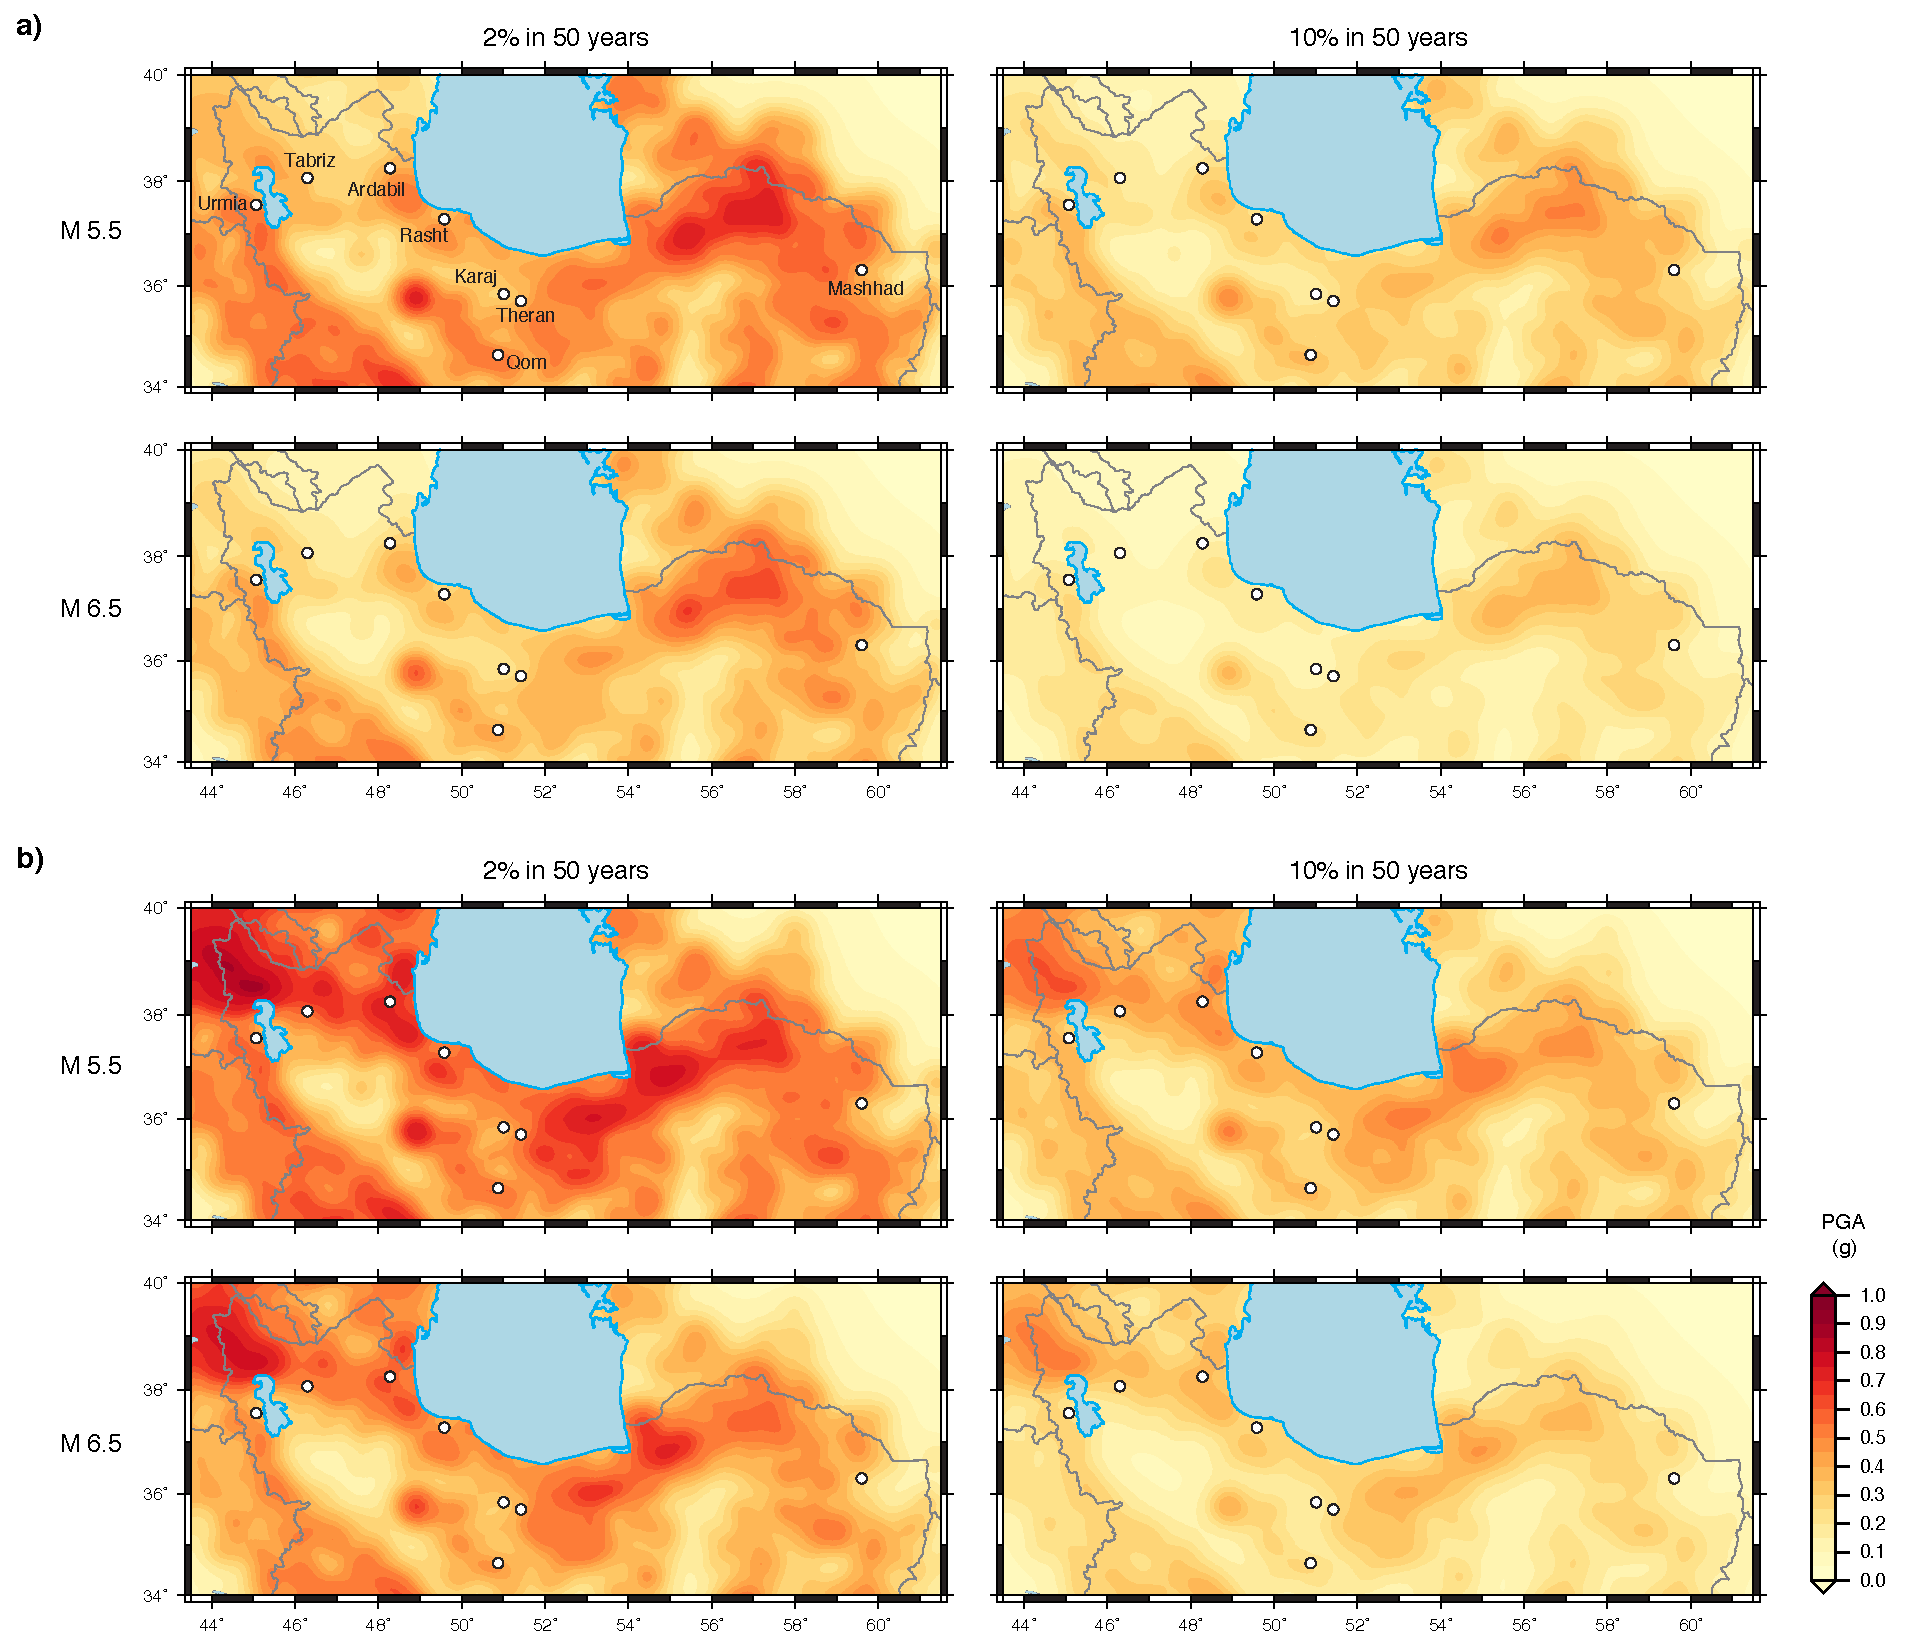
\includegraphics[width=\textwidth]{figures/pdf/figure-08.pdf} 
    \caption{Expected mean peak ground acceleration (PGA) for 2 and 10 percent of probability of exceeding earthquake magnitudes $M_w$ 5.5 and 6.5 for (a) the five seismic regions R model and (b) the uniform seismic region U model.}
    \label{fig:pga}
\end{figure*}

\begin{figure*}[t]
    \centering
    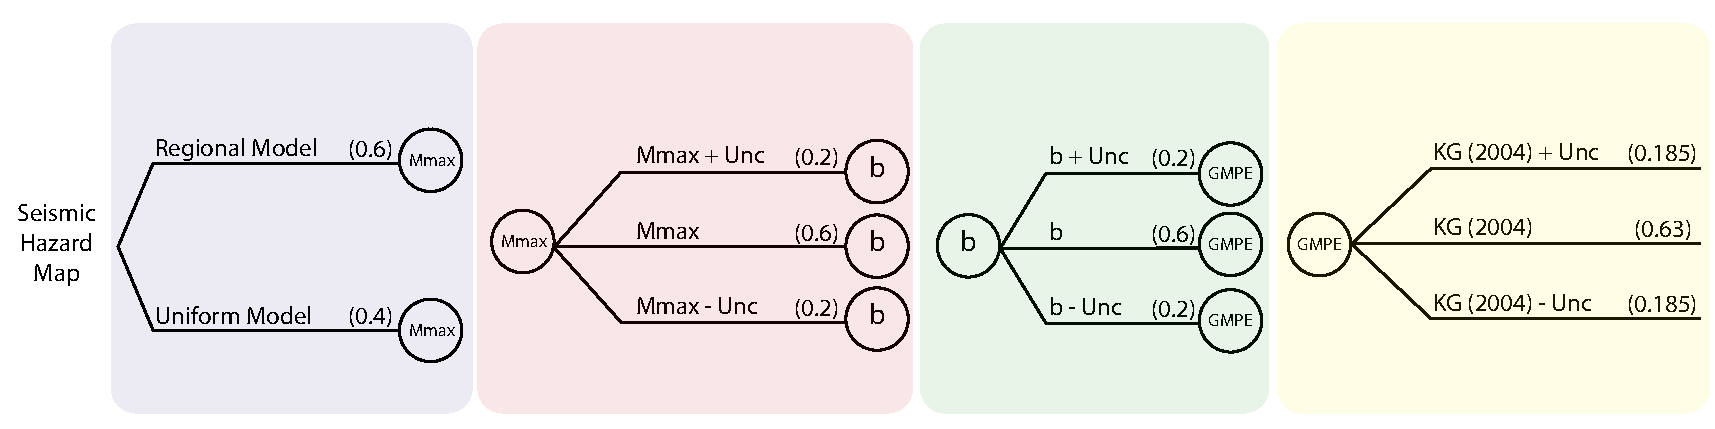
\includegraphics[width=\textwidth]{figures/pdf/figure-09.pdf} 
    \caption{Difference between the mean PGA values obtained for the uniform U model results and the corresponding R models for 2 (left) and 10 (right) percent probabilities of exceeding magnitudes $M_w$ 5.5 (top) and 6.5 (bottom).}
    \label{fig:pgadiff}
\end{figure*}

\begin{figure*}[t]
    \centering
    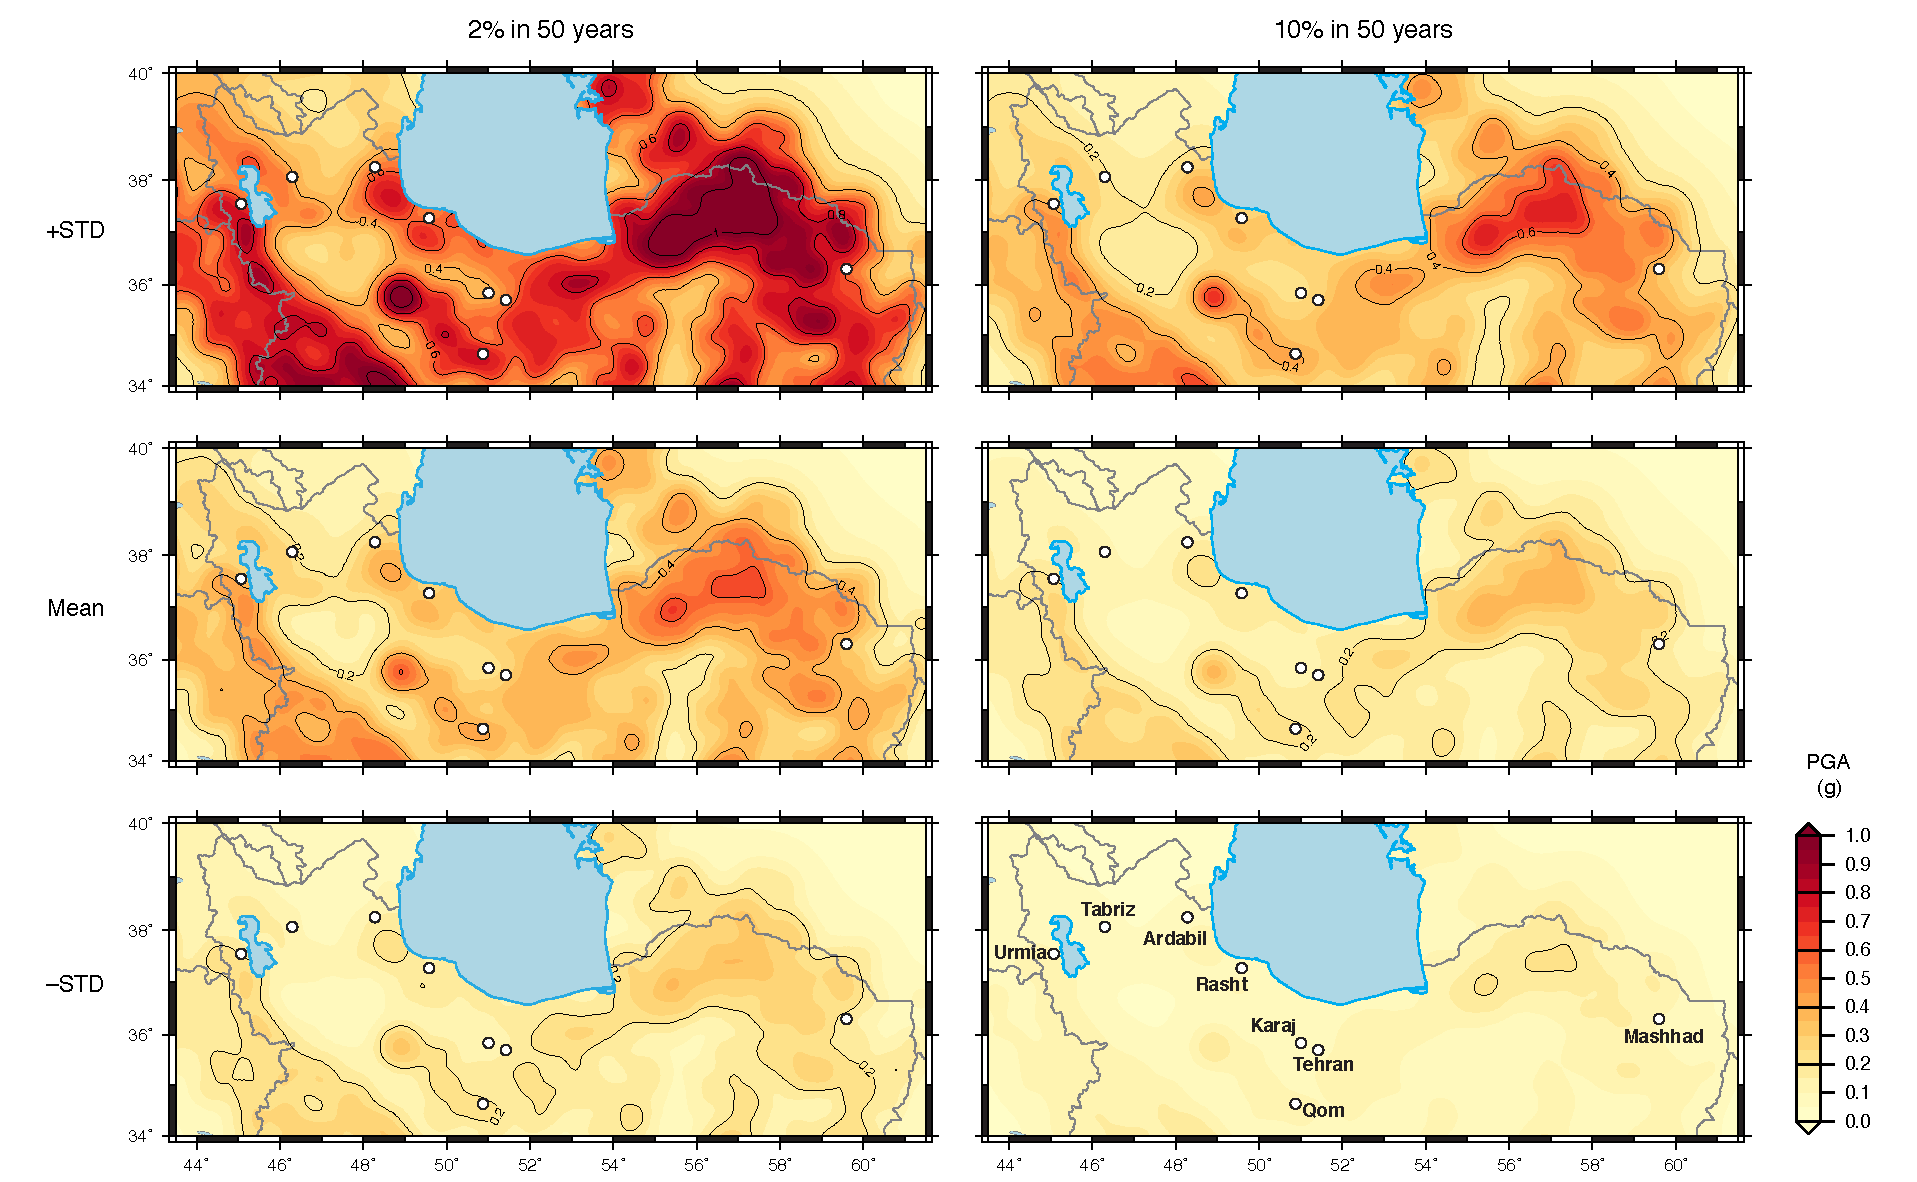
\includegraphics[width=\textwidth]{figures/pdf/figure-10.pdf} 
    \caption{Expected PGA values throughout the region of interest for 2 and 10 percent probability of exceeding an earthquake magnitude $M_w$ 6.5 using the hazard calculations from the five-region R model and the attenuation relationship plus and minus one standard deviation.}
    \label{fig:pgastd}
\end{figure*}

\begin{figure*}[th!]
    \centering
    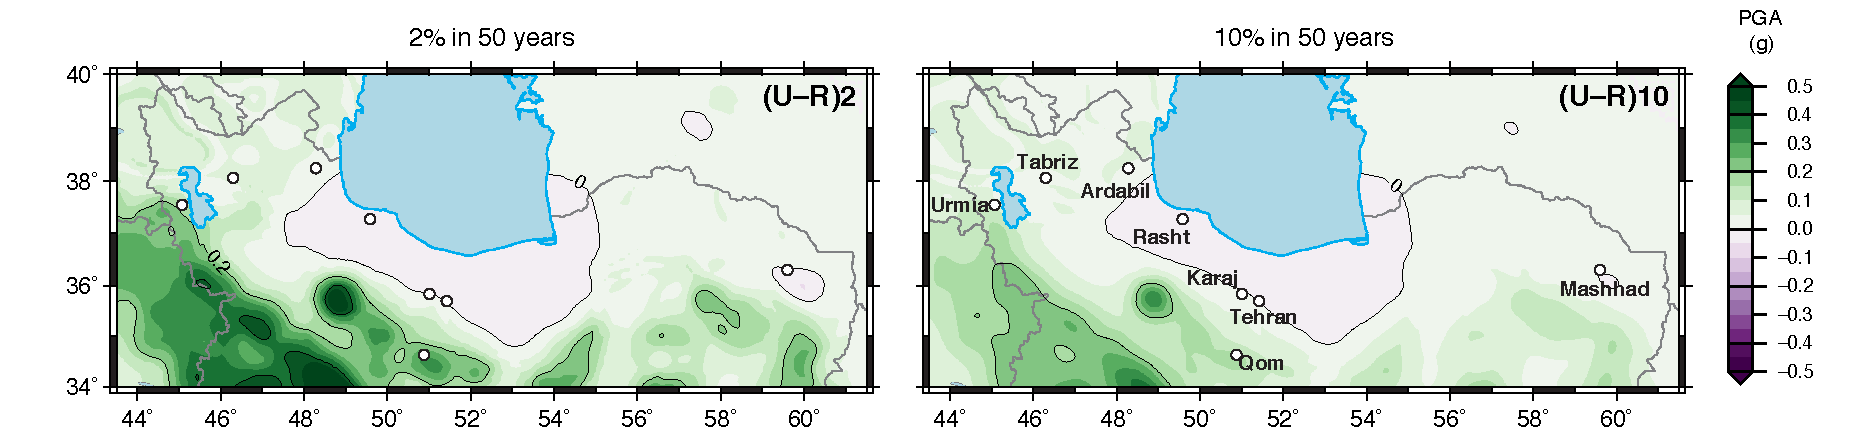
\includegraphics[width=\textwidth]{figures/pdf/figure-11.pdf} 
    \caption{Expected PGA values for different combination models. (a) Combination of R models for magnitudes $M_w$ 5.5 and 6.5. (b) Combination of U models for magnitudes $M_w$ 5.5 and 6.5. (c) Combination of R and U models for separate magnitudes $M_w$ 5.5 and 6.5. (d) Combination of R and U models, and magnitudes $M_w$ 5.5 and 6.5.}
    \label{fig:pgaavgs}
\end{figure*}

\section{Results and Analysis}

Using the data, parameters, and procedures described above, we considered different hazard models based on whether we use the five distinct seismic hazard regions or the whole area of interest as a uniform seismic hazard region. We call these the R and U models, respectively. We also considered two threshold levels of ground motion for events exceeding magnitudes $M_w$ 5.5 and 6.5. We refer to these models with the suffixes 5.5 and 6.5, respectively. Each of these are considered under two probabilities of exceedance, at 2 and 10 percent in 50 years, for which we use the prefixes 2 and 10, respectively. These probabilities correspond to return periods of 475 and 2475 years. As an example of the chosen nomenclature, we refer to the results for 2 percent probability of exceeding an event magnitude $M_w$ 5.5 in 50 years under the five seismic regions model as the 2R5.5 model results.

In the distinct regions R models, we computed the probability of exceedance of the ground motion separately for each region and then added their exceedance rates at a given level of ground motion in order to have the contribution of all regions for any given grid point within the region of interest. The results are obtained in the form of annual rate of exceedance. Expected PGA values are therefore a ``slice'' of the actual hazard curves cut across all grid points for a chosen exceedance rate.

We extract expected levels of ground motion for magnitudes 5.5 and 6.5, based on the assumption that buildings of different construction systems may be vulnerable to different magnitude earthquakes. It is natural to anticipate that modern constructions in urban areas in Iran follow current building regulations and are thus well-designed to withstand moderate magnitude earthquakes $M_w$ 4.5--6.5, and to undergo moderate non-life threatening damage during $M_w > 6.5$ events. Unconventional constructions in poor city outskirts, rural housing and historical buildings may, however, be vulnerable to $M_w \leq 5.5$, and thus becomes relevant to entertain lower magnitude exceedance levels. In turn, the 2 and 10 percent probability of exceedance in a 50-years span are considered a standard practice in seismic design \citep[e.g.,][]{BHRC2014}.

Fig.~\ref{fig:pga} shows the expected mean PGA values obtained using the selected attenuation relationship as a measured of gravity (g) throughout the region of interest for the different model combinations. As can be expected, the highest levels of ground motion are associated with the 2R5.5 and 2U5.5 models, and the lowest with the 10R6.5 and 10U6.5 models. In results for the R models shown Fig.~\ref{fig:pga}a, the highest levels of expected ground motion occur in the Kopeh Dagh region along the border with Turkmenistan, and in a small area half-way between the city of Karaj and the Piranshahr fault, where a small concentration of events can be observed in Fig.~\ref{fig:catalog}b, as well as along the Piranshahr and Morvarid fault lines between the Zagros and Azerbaijan seismic regions (see Fig.~\ref{fig:selected}a for reference). The Azerbaijan seismic zone does not present equally high levels of expected ground motion. In the U models shown in Fig.~\ref{fig:pga}b, on the other hand, the highest levels of expected ground motion are observed precisely in the area corresponding to the Azerbaijan seismic region, especially in the vicinity of the North Tabriz Fault system (see Fig.~\ref{fig:selected} for reference).

In general, the U models exhibit higher levels of expected ground motions when compared to their corresponding R models. This is illustrated in Fig.~\ref{fig:pgadiff}, which shows the differences between both set of models, U--R (U minus R). In this figure, positive values indicate that the U models have larger mean PGA values than the R models. As it can be seen, this is true practically throughout the whole region at very low levels, and in particular in the north-central region at a moderate level of up to 0.2 g and most predominantly in the north-western region of Azerbaijan at levels of about 0.2 to 0.5 g.

Overall, these results are consistent with the seismicity observed in Fig.~\ref{fig:catalog}. The R model results, however, seem to be more sensitive to the influence of large magnitude events observed in both the historical and modern seismicity maps, with concentration of strong earthquakes in the Alborz and Kopeh Dagh regions; whereas the U model results seem to be more sensitive to the influence of low-to-moderate magnitude events, especially in the Azerbaijan region. This is because of the higher $b$-value obtained for the Azerbaijan region in the R model as opposed to the lower value for the U model.

These, of course, are only mean expected levels of ground motion. A more complete picture is captured when considering statistical deviations. Fig.~\ref{fig:pgastd} shows again the mean PGA for the models 2R6.5 and 10R6.5, but this time along with the marginal values of plus and minus one standard deviation. Here, the standard deviation is carried forward in the calculation from the attenuation relationship and thus affects every grid point differently depending on the added contributions from each region. 

The highest expected PGA values are observed in the 2R6.5+STD model with accelerations of higher than 1 g in the Kopeh Dagh region and west of Tehran, and 0.8 g south of the North Tabriz Fault system and in the Zagros region along. These maximum values should, nonetheless, be interpreted with caution given the fact that predictions are based on rock-site assumptions and do not include any kind of site effects, such as inelastic deformation of near-surface geotechnical layers which may often contribute to mitigate peak accelerations.

An additional consideration to make here is the fact that any one model cannot be uniquely correct. They all carry a certain level of epistemic uncertainty which makes them equally accurate and inaccurate at the same time. A means to address the uncertainty intrinsic to each model is to use combinations of different models. We consider different types of combinations to aid our analysis. First, we combine results at in the R and U models independently by averaging the two magnitude results. These combinations follow the hypothesis that in areas where mixed reinforced and unreinforced buildings are present, the hazard and associated expected ground motions will be an average of both magnitude thresholds. Fig.~\ref{fig:pgaavgs}a shows the result of this combination for the R models and Fig.~\ref{fig:pgaavgs}b shows the result for the combined U models. Second, we consider the combination of the two underlying hazard models R and U for the separate magnitude levels. These results are shown in Fig.~\ref{fig:pgaavgs}c. Last, we consider an overall combination of both hazard models and magnitude thresholds, as shown in Fig.~\ref{fig:pgaavgs}d.

These figures show interest results. Combining the two magnitude levels in either the R or U models (Figs.~\ref{fig:pgaavgs}a and \ref{fig:pgaavgs}b) does not have a significant impact other than finding a middle point in between the two ``slices'' taken at the corresponding hazard curves of all the individual grid points. For that matter, defining a threshold at $M_w$ 6.0 is almost equivalent and becomes only a matter of choice. Combining both R and U models, and the two magnitude results (Fig.~\ref{fig:pgaavgs}d), on the other hand, oversmooths the results and eliminates some of the detail desirable in this kind of analysis. It is therefore the combination of the R and U models, but at the separate magnitude thresholds (Fig.~\ref{fig:pgaavgs}c) the one that offers the most plausible scenario. These combinations are the ones that best match the visual inspection of the seismicity of the region (shown in Fig.~\ref{fig:catalog}) and follow the major faults (shown in Fig.~\ref{fig:selected}a), while also bringing into the picture the regional background seismicity of moderate magnitude earthquakes. That is, in the combinations shown in Fig.~\ref{fig:pgaavgs}c one can clearly observe the contribution of the North Tabriz Fault system in the Azerbaijan region, the contribution of the Piranshahr and Morvarid faults in the Zagros region, and that of the different faults in the Alborz and Kopeh Dagh regions. 

\setlength{\tabcolsep}{1ex}

\begin{table*}[t]
\centering
\caption{Comparison of expected PGA values (in $g$) for selected cities in northern Iran between results obtained in this study and those of others previous studies. In our results, the values of the R and U models correspond to mean PGA values as shown also in Fig.~\ref{fig:pga}, and the (R,U) model values correspond to the combination of the R and U models shown in Fig.~\ref{fig:pga.ru.std}. The following codes are used for the references of other studies.
    Gh03: \citet{Ghodrati2003},
    Gh08: \citet{Ghodrati2008},
    Va11: \citet{Vafaie2011},
    Za12: \citet{Zare2012},
    Ab13: \citet{Abdi2013},
    BC14: \citet{BHRC2014},
    Go14: \citet{Golara2014},
    Az14: \citet{Abdollahzadeh2014a},
    Bo15: \citet{Boostan2015}.
    Kh16: \citet{Khodaverdian_2016_BSSA}
    }
\begin{tabular}{lccccccccc}
    \hline                                                                                                              \\[-1.6ex]
    \multicolumn{2}{l}{This study}
                     && \multicolumn{7}{c}{City (lat., lon.)}                                                           \\[0.6ex]
    \cline{4-10}                                                                                                        \\[-1.6ex]
            &        &&   Urmia     &   Tabriz    &   Ardabil   &   Rasht     &   Karaj     &   Tehran    &   Mashhad   \\
    Model   & Prob.  && (45.1,37.6) & (46.3,38.1) & (48.3,38.3) & (49.6,37.3) & (51.0,35.8) & (51.4,35.7) & (59.6,36.3) \\[0.6ex]
    \cline{1-2} \cline{4-10}                                                                                            \\[-1.6ex]
    R       &  10\%  &&   0.21      &   0.35      &   0.44      &   0.37      &   0.25      &   0.31      &   0.22      \\
            &   2\%  &&   0.35      &   0.60      &   0.73      &   0.61      &   0.41      &   0.53      &   0.39      \\
    U       &  10\%  &&   0.28      &   0.39      &   0.48      &   0.35      &   0.25      &   0.31      &   0.22      \\
            &   2\%  &&   0.50      &   0.67      &   0.76      &   0.58      &   0.42      &   0.53      &   0.38      \\
    (R,U)   &  10\%  &&   0.24      &   0.35      &   0.43      &   0.34      &   0.25      &   0.31      &   0.22      \\
            &   2\%  &&   0.38      &   0.61      &   0.73      &   0.58      &   0.40      &   0.53      &   0.39      \\
    \hline                                                                                                              \\[-1.6ex]
    \multicolumn{2}{l}{Other Studies}                                                                                   \\[0.6ex]
    \cline{1-2} \cline{4-10}                                                                                            \\[-1.6ex]
    Kh16    &  10\%  &&  0.15--0.20 & 0.15--0.20  & 0.30--0.35  & 0.15--0.20  & 0.15--0.20  & 0.15--0.20  & 0.10--0.15  \\
            &   2\%  &&  0.30--0.40 & 0.30--0.40  & 0.60--0.70  & 0.30--0.40  & 0.30--0.40  & 0.30--0.40  & 0.20--0.30  \\
    Bo15${}^{*}$
            &  10\%  &&   --        &   --        &   --        &   --        &   --        & 0.38--0.48  &   --        \\
    Az14    &  10\%  &&   --        &   --        &   --        & 0.25--0.30  &   --        &     --      &   --        \\
            &   2\%  &&   --        &   --        &   --        & 0.55--0.60  &   --        &     --      &   --        \\
    BC14    &  10\%  &&   0.30      &   0.35      &   0.30      &   0.30      &   0.35      &   0.35      &   0.30      \\
    Go14    &   2\%  && 0.30--0.50  & 0.90--1.20  & 0.50--0.70  & 0.50--0.70  & 0.70--0.90  & 0.70--0.90  & 0.70--0.90  \\
    Ab13${}^{*,\dagger}$
            &  10\%  &&   --        &   --        &   --        &   --        &   0.31      & 0.27--0.30  &   --        \\
            &   2\%  &&   --        &   --        &   --        &   --        &   0.42      &     --      &   --        \\
    Za12    &  10\%  && 0.35--0.50  & 0.35--0.50  & 0.35--0.50  & 0.50--0.65  & 0.35--0.50  & 0.35--0.50  & 0.35--0.50  \\
    Va11    &  10\%  &&   --        & 0.20--0.65  &   --        &   --        &   --        &     --      &     --      \\
            &   2\%  &&   --        & 0.30--0.90  &   --        &   --        &   --        &     --      &     --      \\
    Gh08    &  10\%  &&   --        &   --        &   --        &   0.10      &   --        &     --      &     --      \\
            &   2\%  &&   --        &   --        &   --        &   0.20      &   --        &     --      &     --      \\
    Gh03    &  10\%  &&   --        &   --        &   --        &   --        &   --        & 0.32--0.42  &     --      \\
    \hline                                                                                                              \\[-1.6ex]
    \multicolumn{10}{l}{\small{${}^{*}$ Used surface-wave magnitude $M_s$ 4.0 as magnitude threshold}}                  \\
    \multicolumn{10}{l}{\small{${}^{\dagger}$ Used $M_s$ 5.5 and 6.0 for Central-East and Alborz-Azerbaijan as magnitude threshold}}
\end{tabular}
\label{tab:pga}
\end{table*}


We also note that the overall distribution of PGA values shown in Fig.~\ref{fig:pgaavgs}c are the ones that best agree with the recent study by \citet{Khodaverdian_2016_BSSA}. These estimates also agree, on average, with other previous studies. For the north-west seismic regions of Azerbaijan and Zagros, for instance, \citet{Tavakoli1999} predicts maximum mean PGA (10\% in 50 years) values of 0.45 g near the North Tabriz Fault and the North Tehran Fault zones, where we find equivalent values to be between 0.2 and 0.4 g. The results from \citet{Vafaie2011} for the city of Tabriz, on the other hand, are slightly higher than the averages shown in Fig.~\ref{fig:pgaavgs}c and are closer to those we present in Fig.~\ref{fig:pga}b, which are in the order of 0.8 and 0.6 g for the models 2U5.5 and 10U5.5. In the north-central region of Alborz, \citet{Ghodrati2003} and \citet{Boostan2015} predict PGA values of the order 0.27--0.46 g and 0.42--0.48 for Tehran, where we found equivalent results to be between 0.2 and 0.35 g, which are closer to the values reported by \citet{Abdi2013}, who predicts PGA values in the vicinity of Karaj and Tehran to be on the order of 0.3 g. Results from \citet{Ghodrati2008} for the Gilan province around the city of Rasht are also of the same order of those we show in Figs.~\ref{fig:pga} and \ref{fig:pgaavgs}c. Finally, for the Kopeh Dagh region, and in particular, for the city of Bojnurd in the northeast province of Khorasan, \citet{Rahgozar2012} reports expected PGA values for return periods of 475 and 2475 years in range of 0.15--0.22 g and 0.28--0.49 g, respectively, where for magnitudes exceeding $M_w$ 6.5 we found equivalent values to be in the order of 0.2--0.4 and 0.4--0.6 g. 

\begin{figure*}[th!]
    \centering
    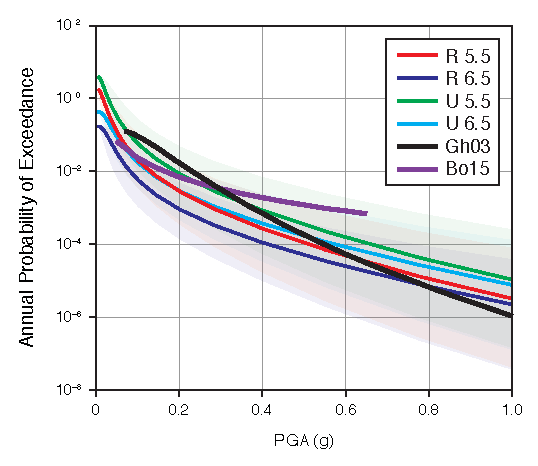
\includegraphics[width=\textwidth]{figures/pdf/figure-12} 
    \caption{Hazard curves representing the annual probability of exceedance as function of peak ground acceleration for six cities in northern Iran based on the four basic models considered in this study, namely R5.5, R6.5, U5.5 and U6.5.}
    \label{fig:hazardcurve}
\end{figure*}

\begin{figure}[t]
    \centering
    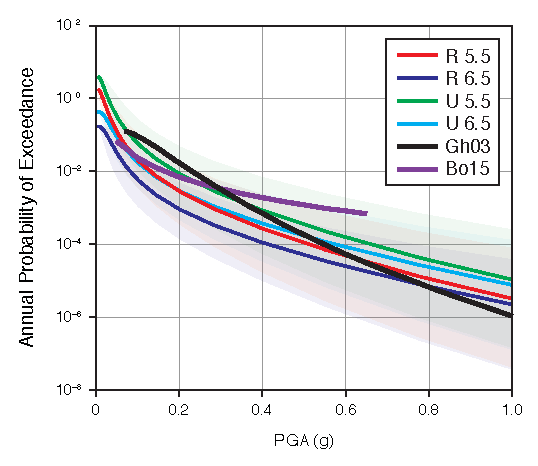
\includegraphics[width=\columnwidth]{figures/pdf/figure-13} 
    \caption{Hazard curve comparison between the models considered in this study and the results of two previous studies by \citet{Ghodrati2003} and \citet{Boostan2015} for the city of Tehran. Here, the two previous studies just mentioned are identified with the codes Gh03 and Bo15, respectively.}
    \label{fig:tehran}
\end{figure}

Table \ref{tab:pga} shows a condensed version of these comparisons between our results and those of other previous studies for selected cities in northern Iran. As mentioned before, overall, our results are close or within the ranges from most studies. The only noticeable exceptions are the results of \citet{Golara2014}, whose expected PGA values are significantly higher the rest, especially in the cities of Tabriz, Karaj, Tehran and Mashhad. This is likely due to the authors working with lower magnitude thresholds (not clearly reported) than other studies where hazard is usually estimated based on earthquake magnitudes exceeding $M_w > 5$. Although not included here for brevity, we also computed expected PGA values for magnitude thresholds $M_w$ 4.5 and 5.0. We found the former case to yield results closer to those of \citet{Golara2014}, but not to the other studies. Using lower magnitude thresholds may be of relevance if evaluating poorly constructed and unreinforced buildings vulnerable to low-to-moderate magnitude earthquakes. We should also note that, in general, the smoothed seismicity method used here tends to lead to lower hazard estimations than those obtained using specific fault definitions (as opposed to point sour\-ces).

Following the comparisons shown in Table \ref{tab:pga}, we looked into the more complete picture of the annual probabilities of exceedance as functions of PGA. The results are shown in Fig.~\ref{fig:hazardcurve} for six of the main cities in northern Iran considering the four basic models R5.5, R6.5, U5.5 and U6.5. In each case we also show $\pm 1$ standard deviation (shaded ranges). These hazard curves exemplify again the differences between the R and U models, which are more prominent in the northwest cities of Tabriz and Ardabil, where the U models yield higher expected values of PGA for any given annual probability of exceedance. Minor differences are also present in the results of the central cities of Karaj and Tehran, whereas for the cities of Urmia and Mashhad in the Zagros and Kopeh Dagh seismic zones, the R and U models yield similar hazard levels. This is consistent with our previous observations regarding Figs.~\ref{fig:pga}, \ref{fig:pgadiff} and \ref{fig:pgaavgs}.

Last, we put additional attention on the results for the capital city of Tehran. We compare hazard curves obtained in this study against those computed by \citet{Ghodrati2003} and \citet{Boostan2015}. Our results are similar to those obtained by \citet{Ghodrati2003} between 0.4 and 0.8 g (corresponding to annual probabilities of exceedance between $10^{-5}$ and $10^{-3}$), but we obtain lower probabilities for the ground motion amplitudes between 0.1 and 0.4 g, and higher probabilities for very low ($<0.1$ g) and much higher PGA ($>0.8$ g) values. These differences with \citet{Ghodrati2003}, nonetheless, are still within our levels of uncertainty. A similar interpretation can be made for the comparison with \citet{Boostan2015} for low PGA values ($<0.4$ g), but the trajectory of their hazard curve suggests much higher probabilities of exceeding PGA values above 0.6 g, which is contrary to our findings.

% ==================
% OLD STUFF NOT USED
% ==================

% The results are presented as annual rate of exceedance. 

% Regarding the study domain and the 0.1 grid size, the total number of source as grid points is 13561. 

% Regarding the study domain and the 0.1 grid size, the total number of source is grid sites is 11651. 

% Even though \citet{Kalkan2004} derived the attenuation relationship up to 250 km, since \citet{Zafarani2014} used data up to 200 km to evaluate the GMPEs, we set the model to compute the ground motions at distances of less than 200 km.

% We pick the peak ground acceleration for 10\% and 2\% probability of exceedance in 50 years which correspond with 0.002 and 0.0004 annual rate of exceedance. 

% \citet{Abdollahzadeh2014a} carried out a probabilistic seismic hazard assessment for part of Northern Iran. They used the logic tree approach to capture the epistemic uncertainty of seismic hazard assessment in delineation of seismic sources and selection of attenuation relationship. They used three attenuation relationships and 2 seismic source models. They collected the earthquake catalog from various references and reported the pga for 475 and 2475 years of return period for northern cities.   

% \citet{Golara2014} conducted a probabilistic seismic hazard analysis of interconnected infrastructure of Iranian high pressure gas supply system. He used line and area source model in order to estimate the Iranian  high-pressure gas supply system's ability to withstand a sudden large ground movements caused by potential earthquakes and related phenomenon that might be expected. he used simplified tectonic map after \citet{Alavi1991}. He used four attenuation relationships and presented the results for 2475 years of return period. 

% The areas of large probabilistic ground motions clearly coincide with zones with a large number of events of magnitude 3.0 and larger. In this study we used two models for seismic hazard calculation, including $M_w>5$ and $M_w>4.5$. $M_w$ is the minimum magnitude that can affect the engineering site. 

% In the probabilistic seismic hazard analysis increasing minimum magnitude will decrease the mean rate of earthquake occurrence ($\nu=exp(\alpha - \beta M_0)$), and also increase the value for the probability density function in the initial magnitudes. In a simple source the difference between different models specially in higher pga levels is negligible. However, in this study where we consider each event as a seismic source with different $\alpha$ and $\beta$ value, the results are considerably different. According to our results the reduction of the mean rate of earthquake occurrence has considerable effect on the results. 
